\chapter{Si spieghi come possiamo calcolare la distanza di edit tra due stringhe v e w utilizzando la griglia dove gli archi sono pesati. Come si ricostruisce una matrice di allineamento che riflette la distanza di edit?}

La \textbf{distanza di edit} è definita come il numero minimo di operazioni elementari (delezione, inserzione, sostituzione) necessarie per trasformare una stringa nell'altra.
\begin{equation}
    d_E(v, w) = \text{numero minimo di operazioni per trasformare } v \text{ in } w
\end{equation}

\textbf{Esempio di trasformazione}

\textbf{TGCATAT} $\rightarrow$ \textbf{ATCCGAT} in 4 passi:
\begin{itemize}
  \item TGCATAT \quad $\rightarrow$ (inserisco \textcolor{blue}{A} all'inizio)
  \item \textcolor{blue}{A}TGCATAT \quad $\rightarrow$ (sostituisco \textcolor{red}{C} al posto della 3$^\circ$ \textcolor{red}{G})
  \item AT\textcolor{red}{C}CATAT \quad $\rightarrow$ (sostituisco \textcolor{red}{G} al posto della 5$^\circ$ \textcolor{red}{A})
  \item ATCC\textcolor{red}{G}TAT \quad $\rightarrow$ (cancello la 6$^\circ$ \textcolor{cyan}{T})
  \item ATCCG\textcolor{cyan}{A}T \quad (fatto)
\end{itemize}

Per calcolare la distanza di edit $d_E(v, w)$ in modo efficiente si costruisce una \textbf{griglia di edit} (alignment grid) con archi pesati e si applica la \textbf{programmazione dinamica}.

Date due stringhe $v$ e $w$, con $n=|v|$ e $m=|w|$ la \textbf{griglia di edit} è un grafo orientato $G=(V, E)$ di dimensioni 
$(n+1) \times (m+1)$, i cui vertici sono coppie $(i, j)$ con $0 \leq i \leq n$ e $0 \leq j \leq m$.
Ogni vertice, inoltre, rappresenta l'allineamento tra prefissi $v[1..i]$ e $w[1..j]$. 
Il vertice $(0,0)$ è il \textbf{nodo sorgente} mentre $(n,m)$ è lo \textbf{stato finale} (sink).
Gli archi della griglia sono i movimenti permessi sulla griglia e sono etichettati mediante \textbf{funzione di costo}.
Ogni cammino da $(0,0)$ a $(n,m)$ rappresenta un possibile allineamento fra $v$ e $w$, mentre il costo complessivo rappresenta il costo dell'allineamento.
Ogni cammino valido nella griglia da sorgente a sink corrisponde esattamente a un allineamento tra $v$ e $w$. Il costo del cammino (somma dei pesi degli archi) è il numero di operazioni di editing.

I movimenti permessi e i loro pesi (costi) sono:
\begin{itemize}
    \item \textbf{Spostamento verticale} da $(i-1, j)$ a $(i, j)$: corrisponde all'inserimento di un gap (\texttt{-}) nella stringa $w$ (delezione di $v_i$). 
    \item \textbf{Spostamento orizzontale} da $(i, j-1)$ a $(i, j)$: corrisponde all'inserimento di un gap (\texttt{-}) nella stringa $v$ (inserimento di $w_j$).
    \item \textbf{Spostamento diagonale} da $(i-1, j-1)$ a $(i, j)$: corrisponde all'allineamento di $v_i$ con $w_j$. (\textit{match} se $v_i = w_j$, \textit{sostituzione} se $v_i \neq w_j$).
\end{itemize}

Formalmente, la \textbf{funzione di costo} $\delta$ assegna un costo alla coppia di simboli che vengono allineati:
\begin{itemize}
    \item \textbf{Match} (caratteri identici): $\delta(v_i,w_j)=0$ se $v_i = w_j$ (ad esempio $\delta(A,A)=0$), poiché non è richiesta alcuna operazione di modifica.
    \item \textbf{Mismatch} (sostituzione): $\delta(v_i,w_j)=1$ se $v_i \neq w_j$ (ad esempio $\delta(A,C)=1$).
    \item \textbf{Indel} (inserzione o delezione): $\delta(v_i,\text{-})=1$ per una delezione e $\delta(\text{-},w_j)=1$ per una inserzione.
\end{itemize}

Questi costi diventano i pesi degli archi nella griglia di edit:
\begin{itemize}
    \item l'arco verticale da $(i-1,j)$ a $(i,j)$ ha peso $\delta(v_i,\text{-})=1$;
    \item l'arco orizzontale da $(i,j-1)$ a $(i,j)$ ha peso $\delta(\text{-},w_j)=1$;
    \item l'arco diagonale da $(i-1,j-1)$ a $(i,j)$ ha peso $\delta(v_i,w_j)$, quindi $0$ se $v_i = w_j$ e $1$ se $v_i \neq w_j$.
\end{itemize}

\begin{figure}[H]
    \centering
    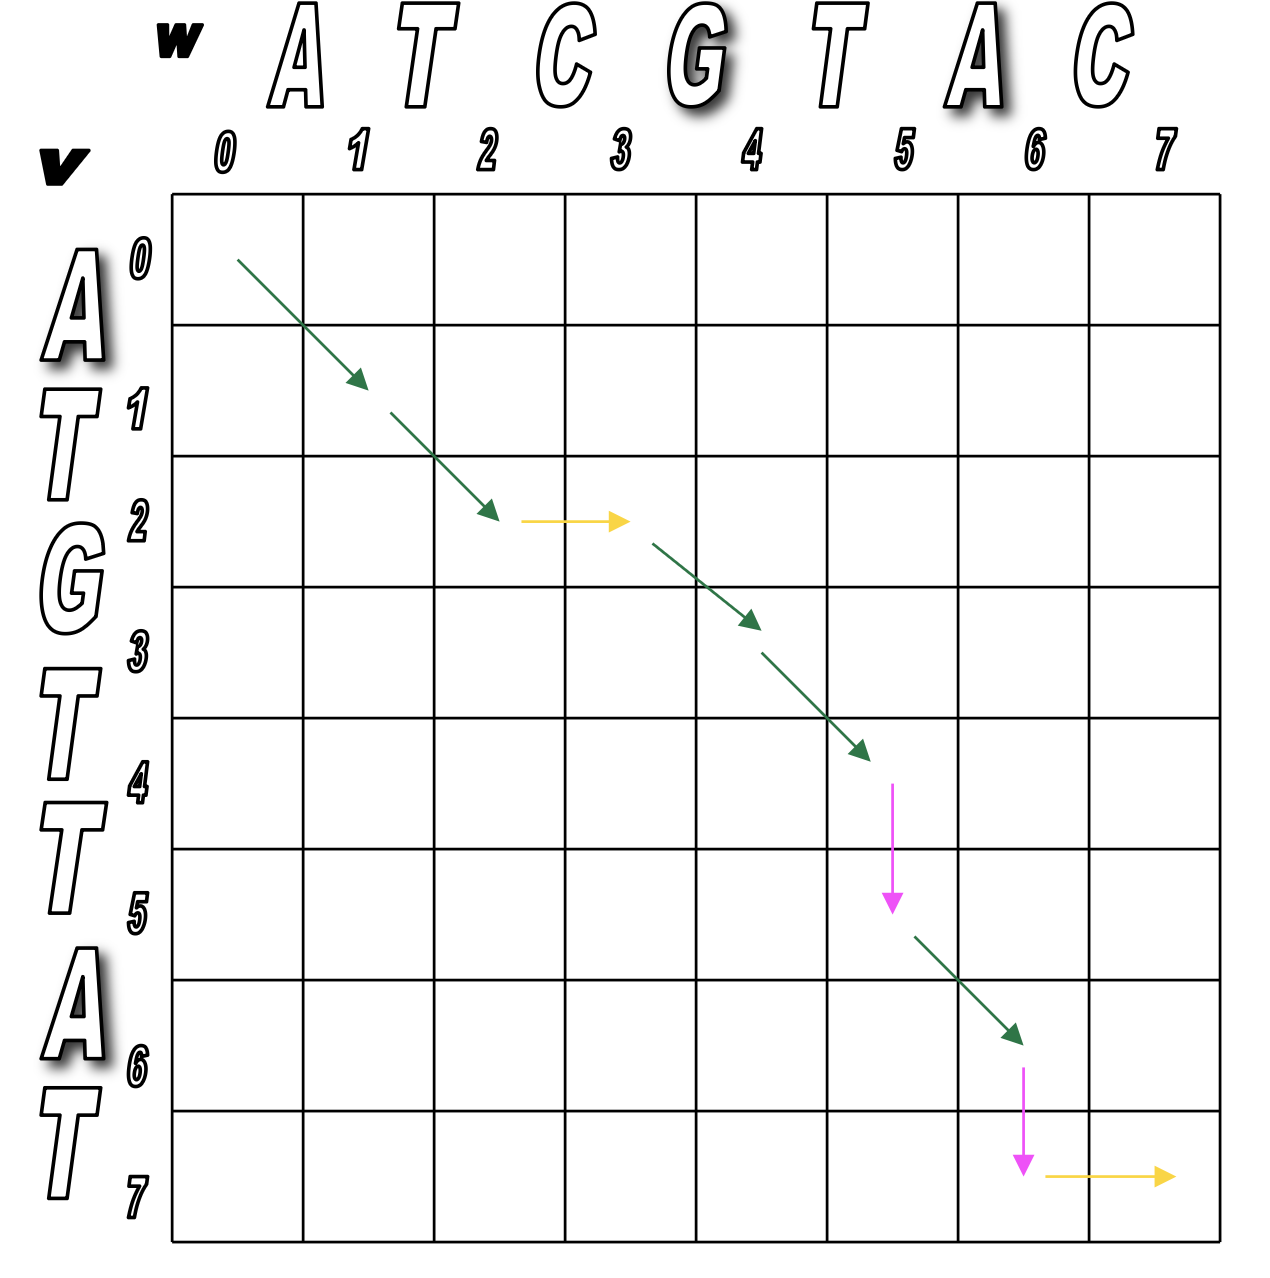
\includegraphics[width=0.7\textwidth]{images/edit_graph.png}
    \caption{Griglia di edit con archi pesati.}
    \label{fig:edit-grid}
\end{figure}

Per calcolare il costo minimo per raggiungere un nodo $(i,j)$ si applica la programmazione dinamica. Prima si definiscono i \textbf{casi base} (inizializzazione della prima riga e prima colonna):
\begin{itemize}
    \item $S(i, 0) = i$ per $0 \leq i \leq n$
    \item $S(0, j) = j$ per $0 \leq j \leq m$
\end{itemize}

Successivamente, si riempie il resto della griglia con la seguente \textbf{equazione di ricorrenza}:
\begin{equation}
    S(i, j) = \min
    \begin{cases}
        S(i-1, j) + 1 & \text{(Delezione)} \\
        S(i, j-1) + 1 & \text{(Inserzione)} \\
        S(i-1, j-1) + \delta(v_i, w_j) & \text{(Match/Mismatch)}
    \end{cases}
\end{equation}
dove $\delta(v_i, w_j) = 0$ se $v_i = w_j$, e $1$ altrimenti.
Il valore calcolato nel nodo \textit{sink}, ovvero $S(n, m)$, rappresenta la \textbf{distanza di edit ottima}. La \textbf{complessità} di calcolo, dovendo valutare un'operazione costante per ogni cella della griglia, è di $\mathcal{O}(n \times m)$ in tempo e in spazio.

\vspace{0.5cm}
\textbf{Ricostruzione della matrice di allineamento}

\begin{figure}[H]
    \centering
    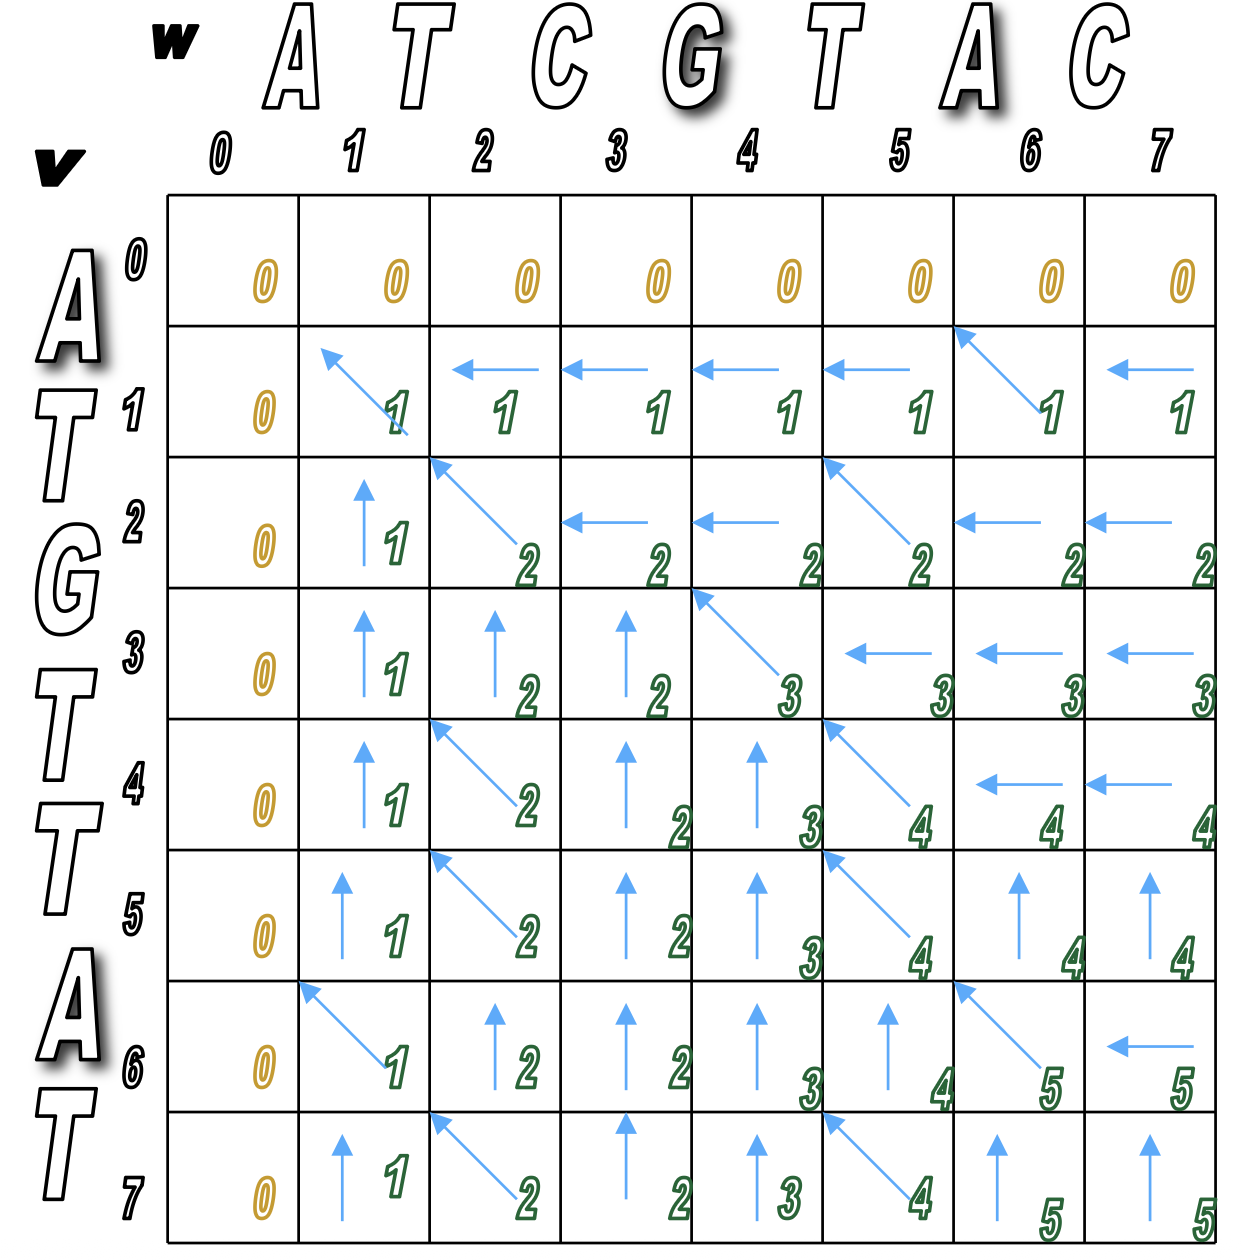
\includegraphics[width=0.7\textwidth]{images/backtracking.png}
    \caption{Backtracking nella griglia per ricostruire un allineamento ottimo.}
    \label{fig:edit-grid-complete}
\end{figure}
Per ricostruire una matrice di allineamento $A$ (di dimensione $2 \times k$, con $k \geq \max(n,m)$) che rifletta tale distanza, si utilizza la procedura di \textbf{backtracking} (percorso a ritroso) all'interno della griglia:

\begin{enumerate}
    \item Si parte dall'ultima cella, ovvero il nodo \textit{sink} $(n, m)$.
    \item Si risale la griglia all'indietro fino ad arrivare al nodo \textit{sorgente} $(0, 0)$. Ad ogni passo, ci si sposta verso la cella adiacente che ha fornito il valore minimo usato nell'equazione di ricorrenza (in caso di parità tra più direzioni ottime, se ne può scegliere una qualsiasi, ottenendo allineamenti alternativi ma con lo stesso score ottimale).
    \item Durante questa risalita, si costruisce la matrice di allineamento aggiungendo una colonna alla volta dall'ultima verso la prima:
    \begin{itemize}
        \item Se lo spostamento a ritroso è \textbf{diagonale} verso $(i-1, j-1)$, si aggiunge la colonna $\begin{pmatrix} v_i \\ w_j \end{pmatrix}$.
        \item Se lo spostamento a ritroso è \textbf{verticale} verso $(i-1, j)$, il carattere $v_i$ è allineato con un gap. Si aggiunge la colonna $\begin{pmatrix} v_i \\ \text{-} \end{pmatrix}$.
        \item Se lo spostamento a ritroso è \textbf{orizzontale} verso $(i, j-1)$, il carattere $w_j$ è allineato con un gap. Si aggiunge la colonna $\begin{pmatrix} \text{-} \\ w_j \end{pmatrix}$.
    \end{itemize}
    \item Il processo termina non appena si raggiunge la cella $(0, 0)$. 
\end{enumerate}

Le colonne così ottenute, lette nell'ordine inverso rispetto a come sono state ricostruite, formano la \textbf{matrice di allineamento globale}. Il \textbf{costo dell'allineamento} si calcola sommando il costo di ogni colonna della matrice:
\begin{equation}
    \text{costo}(A) = \sum_{\ell=1}^{k} \delta(A_{1,\ell}, A_{2,\ell})
\end{equation}
dove ogni colonna $\begin{pmatrix} A_{1,\ell} \\ A_{2,\ell} \end{pmatrix}$ può rappresentare un match, un mismatch oppure un indel. Quindi una colonna con due caratteri uguali ha costo $0$, mentre una colonna con due caratteri diversi oppure con un gap ha costo $1$. La somma dei costi di tutte le colonne coincide con il costo del cammino nella griglia e quindi con la distanza di edit $d_E(v,w)=S(n,m)$.
\newpage
